\chapter{Summary and Outlook}

\subsubsection{Conclusion}

In this thesis, we analyzed several optimization algorithms for the radial reconstruction of images  with a focus on the string art problem. We examined the strengths and weaknesses of each, tuned parameters, and proposed and implemented a new method using the Radon Transform. Our analysis and benchmarks conclude that this approach offers the best balance of reconstruction quality, time and memory efficiency, and stability. For additional tests and detailed results, please refer to Appendix~\ref{app:radon_quantitative}.

\subsubsection{Future work}

In future work, we plan to implement the enhancements to the Radon Transform described in Section~\ref{sec:radon_improvements}. 

Following the modern trend of applying deep learning to classical problems, we experimented with a custom Generative Adversarial Network (GAN) featuring a simplified UNet generator and a custom discriminator to achieve style transfer of string art from normal images. See the results in Figure~\ref{fig:ai}. The code is publicly available at \href{https://github.com/skpha13/stringnet}{stringnet}.

\begin{figure}[H]
    \centering
    \begin{minipage}{0.7\linewidth}
        \centering
        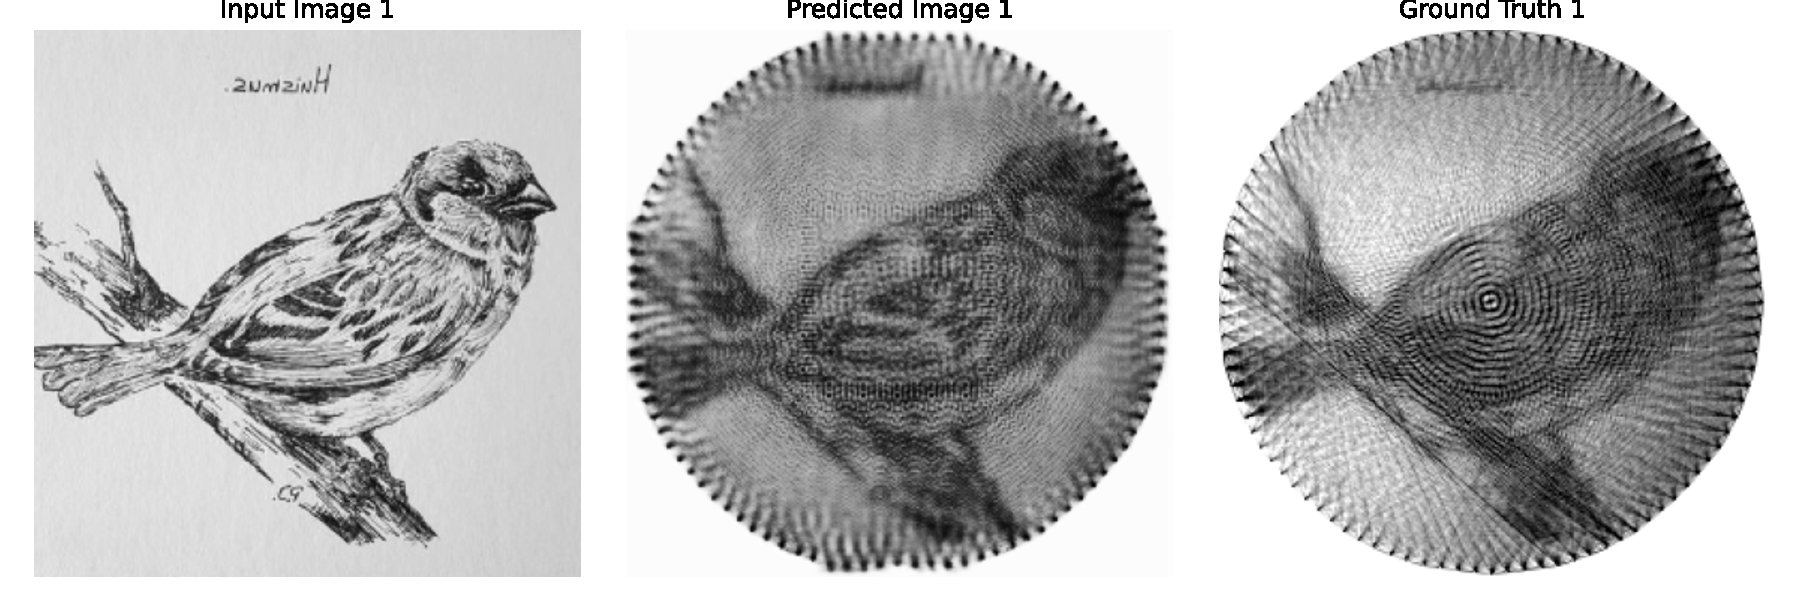
\includegraphics[width=\linewidth]{images/AI/predictions.pdf}
    \end{minipage}%
    \hfill
    \begin{minipage}{0.3\linewidth}
        \centering
        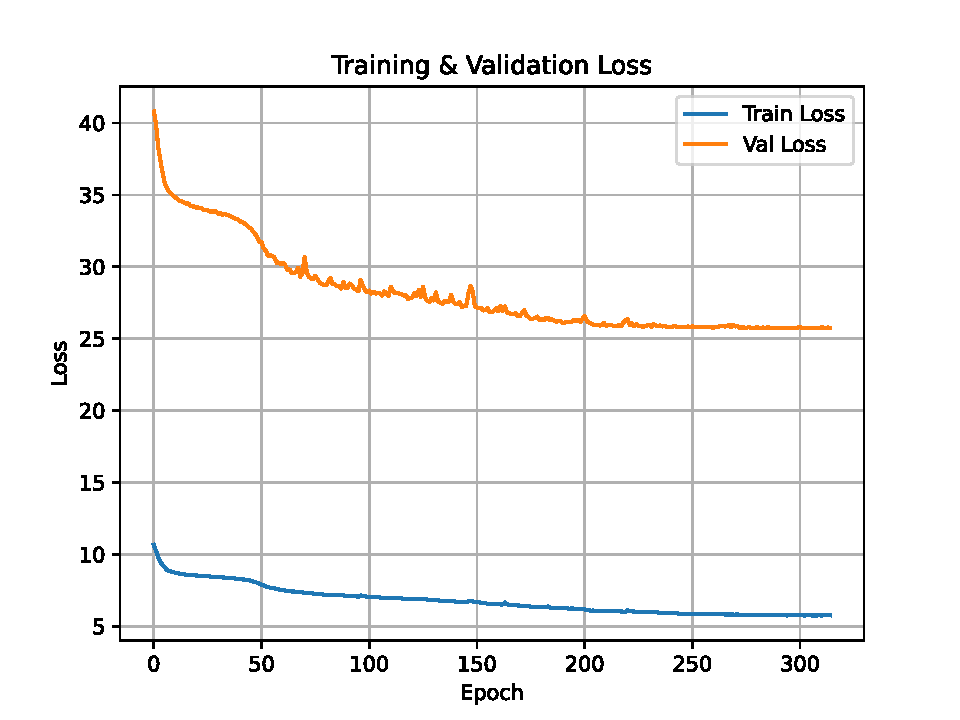
\includegraphics[width=\linewidth]{images/AI/loss.pdf}
    \end{minipage}
    \caption{Results of Generative Adversarial Network for string art image style transfer.}
    \label{fig:ai}
\end{figure}

The idea above works as style transfer, but we could set a fixed number of pegs and then use a deep learning algorithm to find the activation of lines by feeding it input images along with their resulting activation vectors.